\newcommand{\institut}{Institut f\"ur Telekommunikationssysteme}
\newcommand{\fachgebiet}{Nachrichten\"ubertragung}
\newcommand{\veranstaltung}{Praktikum Nachrichten\"ubertragung}
\newcommand{\pdfautor}{Dirk Babendererde (321 836), Thomas Kapa (325 219)}
\newcommand{\autor}{Dirk Babendererde (321 836)\\ Thomas Kapa (325 219)}
\newcommand{\gruppe}{Gruppe:}
\newcommand{\betreuer}{Betreuer: Lieven Lange}


\newcommand{\pdftitle}{Nachrichtenuebertragung\ Praktikum\ 03}
\newcommand{\prototitle}{Praktikum 03 \\ Statistische Nachrichtentheorie}

\input{../../packages/tu_header_8}


% \lstlistoflistings
\definecolor{darkgray}{rgb}{0.95,0.95,0.95}
\definecolor{darkolivegreen}{HTML}{01a801}
\definecolor{functionsBlue}{HTML}{32b9b9}
\definecolor{variableRed}{rgb}{1,0,0}
\definecolor{stringBrown}{HTML}{bc8e8e} % f geht nicht

\lstset{
        %\lstset{extendedchars=true} % Umlaute an der richtigen stelle und nicht am Anfang ausgeben
        %basicstyle=\footnotesize\ttfamily,
        basicstyle=\small,
        %
        inputencoding=utf8,
        %
        tabsize=4,
        showspaces=false,
        showtabs=false,
        showstringspaces=true, % no special string spaces
        %
        backgroundcolor=\color{darkgray}, % background
        stringstyle=\color{stringBrown}\fseries, % Strings
        keywordstyle=\color{functionsBlue}\bfseries, % keywords Blau
        identifierstyle=\color{variableRed}, % variablen
        commentstyle=\color{darkolivegreen}, %  comments
        %
        breaklines=true,
        %
        numbers=left,
        numberstyle=\tiny,
        stepnumber=1,
        numbersep=7pt,
        %
        frame=single,
        columns=flexible,
        %
        xleftmargin=-2cm,
        xrightmargin=-1.5cm,
        %
        language=Matlab,
}
% enables UTF-8 in source code: (dirty, dirty hack)
\lstset{literate=
    %Deutsch
    {ä}{{\"a}}1 {ö}{{\"o}}1 {ü}{{\"u}}1 {Ä}{{\"A}}1 {Ö}
    {{\"O}}1 {Ü}{{\"U}}1 {ß}{\ss}1
    %Türkisch
    {â}{{\^{a}}}1 {Â}{{\^{A}}}1 {ç}{{\c{c}}}1 {Ç}{{\c{C}}}1 {ğ}{{\u{g}}}1 {Ğ}{{\u{G}}}1 {ı}{{\i}}1 {İ}{{\.{I}}}1 {ö}{{\"o}}1 {Ö}{{\"O}}1 {ş}{{\c{s}}}1
    {Ş}{{\c{S}}}1 {ü}{{\"u}}1 {Ü}{{\"U}}1
    %Polish
    {ą}{{\k{a}}}1 {ć}{{\'c}}1 {ę}{{\k{e}}}1 {ł}{{\l{}}}1 {ń}{{\'n}}1 {ó}{{\'o}}1 {ś}{{\'s}}1 {ż}{{\.z}}1 {ź}{{\'z}}1 {Ą}{{\k{A}}}1 {Ć}{{\'C}}1
    {Ę}{{\k{E}}}1 {Ł}{{\L{}}}1 {Ń}{{\'N}}1 {Ó}{{\'O}}1 {Ś}{{\'S}}1 {Ż}{{\.Z}}1 {Ź}{{\'Z}}1
    %Spanish
    {á}{{\'a}}1 {é}{{\'e}}1 {í}{{\'i}}1 {ó}{{\'o}}1 {ú}{{\'u}}1 {ñ}{{\~n}}1
}

%     \lstinputlisting{./praktikum6.sce}



%---------------------------------------------------------------------
%---------------------------------------------------------------------
%---------------------------------------------------------------------


\section{Vorbereitungsaufgaben}
\begin{quote}
    \hspace{-2em}
    \subsection{AM}
        
    \begin{quote}
        
        Da alle Werte eines analogen Signals $\geq 0$ sein Müssen um sie mittels AM mit Träger übertragen zu können, haben wir für
        diesen Versuch mit Matlab Cosinus-, Dreieck- und Rechtecksignale folgenden Eigenschaften erzeugt:
        
        
        \begin{equation*}
        \begin{split}
        \\
                 0 &\leq u(t) \leq 2.0
        \\
                 f &= \si{100}{Hz}
        \\
            \alpha &= 0.5
        \\
                 T &= \si{2}{s}
        \\
               f_T &= \si{1}{MHz}
        \\
        \end{split}
        \end{equation*}
        
        
        Außerdem haben wir noch ein cosinus-Trägersignal mit \si{2}{kHz} erzeugt. Auf dieses Trägersignal haben wir dann, zum
        späteren vergleich, die erzeugten Basisbandsignale raufmoduliert.
        
    \end{quote}
    
    
    
    
    \subsection{FM}
    \begin{quote}
        
        
        Zur Vorbereitung der FM-Modulation haben wir ein Cosinussignal mit folgenden Eigenschaften simuliert.
        
        \begin{equation*}
        \begin{split}
        \\
                 0 &\leq u(t) \leq 2.0
        \\
                 f &= \si{100}{Hz}
        \\
                 T &= \si{0,5}{s}
        \\
               f_T &= \si{1}{MHz}
        \\
        \end{split}
        \end{equation*}
        
        
        Dieses Trägersignal haben wir dann mit einem weiteren cosinus ($f_u = 1kHz$ und $A_u = 1V$) nach der folgenden Formel
        moduliert:
        
        \begin{equation*}
        \begin{split}
        \\
                u_m(t) &= A \p cos(\varphi(t))
        \\
            \varphi(t) &= 2 \pi f_c t + K_{FM} \p \int\limits_{-\infty}^t u(\tau) \ d\tau  
        \\
        \end{split}
        \end{equation*}
        \label{equ:fm}
        
        Von diesem Modulierten Signal ($u_m$) haben wir noch, zum späteren Vergleich, mit Hilfe von Matlab das Amplitudenspektrum
        bestimmt.
        
        
    \end{quote}
    
    
    \subsection{Theorie zur FM-Demodulation}
    \begin{quote}
%         Wir haben im praktikum die FM-PFM-Umwandlung als Methode zur FM-Demodulation genutzt, da es ein relativ einfaches
%         Verfahren ist. Hierbei wird das Signal zunächst durch einen Comparator in eine polare Rechteckfolge umgewandelt. Als
%         Referenz für den Comparator wird \si{0}{\volt} eingestellt, damit jede positive Halbwelle des modulierten Signals zu
%         einem positiven Rechteck wird und jede negative zu einem Negativen.\\
%         Anschließend wird das Signal noch durch einen Twin Pulse Generator geführt, der aus jeder steigenden Flanke ein
%         Rechteckimpuls macht.\\
%         Wofür der Twin Pulse Generator gebraucht wird ist leider weder aus dem Skrip ersichtlich, noch konnte es uns im Praktikum
%         einleuchtend erklärt werden. Er wird wohl ``wegen irgendwelcher Feedback-Sachen oder so''\footnotemark gebraucht.\\
%         Zuletzt wird das Signal noch tiefpass-gefiltert, um aus der Häufigkeit der Pulse wieder das Analoge ausgangssignal zu
%         machen.
%         \footnotetext{Aussage des Tutors im NUE-Praktikum am 16.05.2012}
        
    \end{quote}
    
    
\end{quote}

%--------------------------------------------------------------------
%--------------------------------------------------------------------


\section{AM}
\begin{quote}
    
    
    \subsection{Labordurchführung}
    \begin{quote}
      Das mit Hilfe von Amplitudenmodulation zu übertragende Signal soll ein
      Sinussignal mit Amplitude von 1 V, einer Frequenz von 100 Hz, mittelwertfrei sein und von Funktionsgenerator geliefert 
      werden. Um das Signal von negativen Werten zu befreien (siehe
      Vorbereitung) wird das Signal mit Hilfe des Adder-Moduls und der variablen DC Voltage Quelle
      um ein Volt angehoben. Da das Adder-Modul den Ausgang invertiert, wird der
      Ausgang des ersten Adders auf einen zweiten Adder gegeben und der zweite
      Eingang auf Masse gelegt, um das Signal zu invertieren. //
      Um Trägersignal und das zu übertragende Signal zu überlagern wird das
      Multiplier-Modul verwendet. Dabei liefert das Master-Signal-Modul ein 2
      kHz Sinussignal, das als Trägersignal dient, das mit dem zu übertragenden
      Signal multipliziert wird.
        Mit der Demodulation über einen als idealen betrachteten Kanal kann das
        Signal durch eine erneute Multiplikation mit dem Trägersignal
        zurückgewonnen werden.
        
      \begin{equation*}
        \begin{split}
         y_{d}(t)=u_{m}(t)cos(\omega_{c}t)=u(t)cos^{2}(\omega_{c}t)=\frac{1}{2}u(t)\cdot
         (1+cos(2\omega_{c}t))
         \label{eq:demodulation}
        \end{split}
        \end{equation*}
        
        In Formel \ref{eq:demodulation} kann man erkennen, dass der vordere Teil
        bis auf den Vorfaktor 0,5 dem Basisbandsignal entspricht. Der hintere
        Teil weist eine doppelt so hohe Frequenz auf, die man mit einem
        entsprechend dimensionierten Filter herausfiltern kann.
        Dabei werden auch die Signale nach der Demodulation ohne Tiefpass
        aufgenommen und in der Auswertung mit denen mit Tiefpass verglichen.
        Zuletzt kann man ein zweites Multiplier-Modul hinzufügen und den Ausgang
        von diesem auf einen entsprechenden Tiefpass geben und erhält sein
        Signal zurück.
        
    \end{quote}
    
    
    \subsection{Auswertung}
    \begin{quote}
        Eine Veränderung der Amplitude des Basisbandsignals führt dazu, dass,
        wenn die Amplitude zu groß wird, das Signal Anteile unter 0 bekommt.
        Damit verändert sich die Einhüllende des modulierten Signals und eine
        Rückgewinnung durch Demodulation ist nicht mehr möglich. Ein Beispiel
        ist in Abb. \ref{fig:Ampl} zu sehen, wobei die Amplitude bei 2 V liegt
        und der Offset bei 1 V.
        
    \begin{figure}[H]
		\begin{center}
			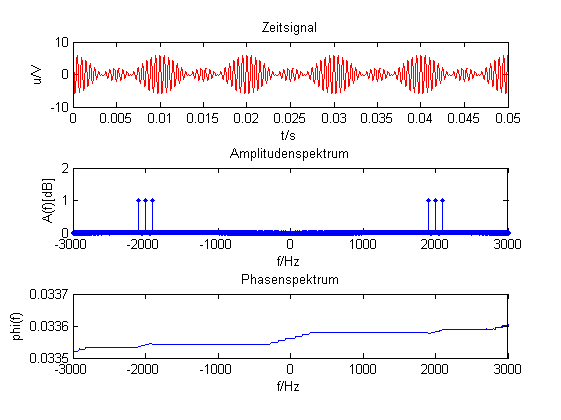
\includegraphics[width=0.8\textwidth]{Bilder/Cos_zugrosseAmpl}
		\end{center}
		\caption{zu große Amplitude des Basisbandsignals}
		\label{fig:Ampl}
	\end{figure}
	
	Bei dem Offset entsteht der selbe Fehler, nur dass dieser nicht zu klein
        sein darf. Abb. \ref{fig:Offs} zeigt die Modulation für eine Amplitude
        von 1 V und einem Offset von 0,2 V.
	
	 \begin{figure}[H]
		\begin{center}
			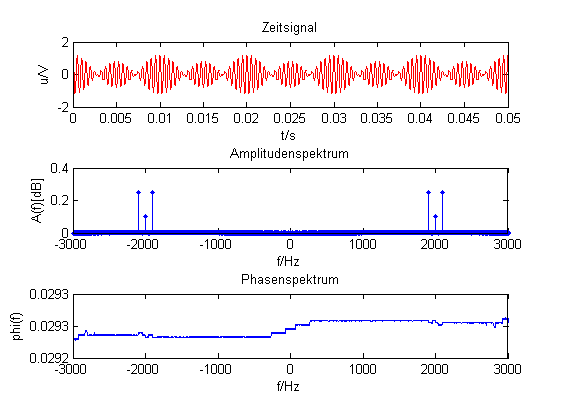
\includegraphics[width=0.8\textwidth]{Bilder/Cos_zukleinerOffset}
		\end{center}
		\caption{zu kleiner Offset des Basisbandsignals}
		\label{fig:Offs}
	\end{figure}
        
        In Abb. \ref{fig:Mocosinussimu} und \ref{fig:Mocosinus} sind sowohl die
        mit Matlab simulierte, als auch die gemessene Modulation eines Cosinus
        abgebildet. Es ist gut zu erkennen, dass die Simulation mit der Praxis
        gut übereinstimmen. Lediglich bei der Amplitude sind versehentlich
        unterschiedliche Werte aufgenommen worden.
        Gut zu erkennen sind jeweils die beiden großen Peaks bei +- 2 kHz des
        Trägersignals und die jeweils um diese 2 kHz um 100 Hz versetzten
        Nebenpeaks des Basisbandsignals.
        
        \begin{center}
        \begin{tabular}{ll}
        
        \hspace{-5cm}
            \begin{minipage}{0.67\textwidth}
                
                \begin{figure}[H]
                    \label{fig:Mocosinussimu}
                    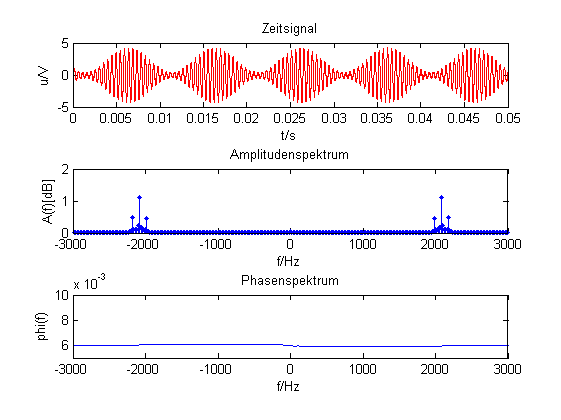
\includegraphics[scale=0.7]{Bilder/Am_Cos_2k_100Hz_mo_simu}
                    \caption{mit Matlab simulierte Modulation eines Cosinus}
                \end{figure}
        
            \end{minipage}
        
            \begin{minipage}{0.67\textwidth}
                \begin{figure}[H]
                    \label{fig:Mocosinus}
                    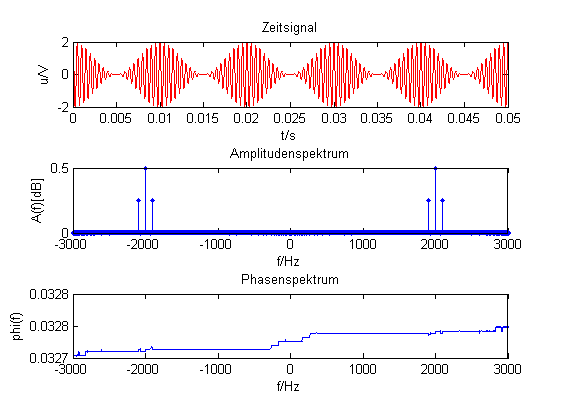
\includegraphics[scale=0.7]{Bilder/Am_Cos_2k_100Hz_mo}
                    \caption{gemessene Modulation eines Cosinus}
                \end{figure}
        
            \end{minipage}
        
        \end{tabular}
        \end{center}
        
        \begin{center}
        \begin{tabular}{ll}
        
        \hspace{-5cm}
            \begin{minipage}{0.67\textwidth}
                
                \begin{figure}[H]
                    \label{fig:Modreiecksimu}
                    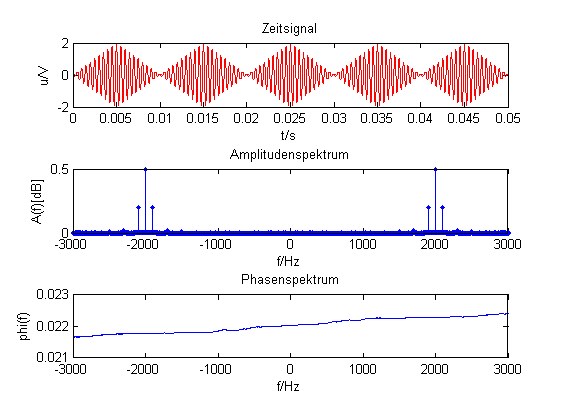
\includegraphics[scale=0.7]{Bilder/Am_Dre_2k_100Hz_mo_simu}
                    \caption{mit Matlab simulierte Modulation eines
                    Dreieck}
                \end{figure}
        
            \end{minipage}
        
            \begin{minipage}{0.67\textwidth}
                \begin{figure}[H]
                    \label{fig:Modreieck}
                    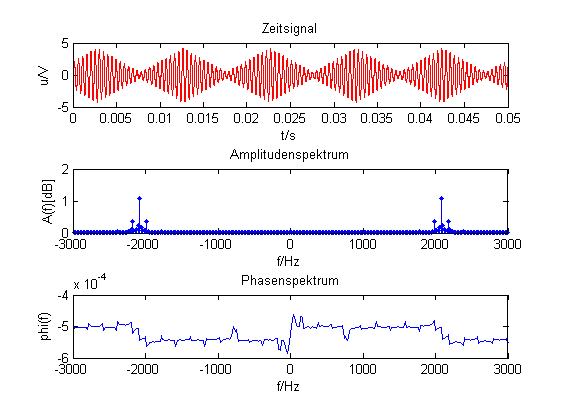
\includegraphics[scale=0.7]{Bilder/Am_Dre_2k_100Hz_mo}
                    \caption{gemessene Modulation eines Dreieck}
                \end{figure}
        
            \end{minipage}
        
        \end{tabular}
        \end{center}
      
        \begin{center}
        \begin{tabular}{ll}
      
        \hspace{-5cm}
            \begin{minipage}{0.67\textwidth}
                
                \begin{figure}[H]
                    \label{fig:Morechtecksimu}
                    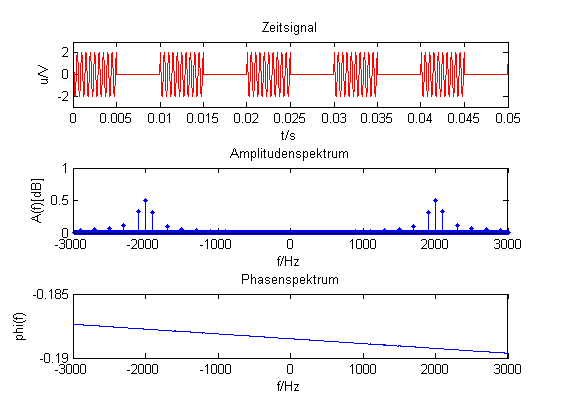
\includegraphics[scale=0.7]{Bilder/Am_Rec_2k_100Hz_mo_simu}
                    \caption{mit Matlab simulierte Modulation eines Rechteck}
                \end{figure}
        
            \end{minipage}
    
            \begin{minipage}{0.67\textwidth}
                \begin{figure}[H]
                    \label{fig:Morechteck}
                    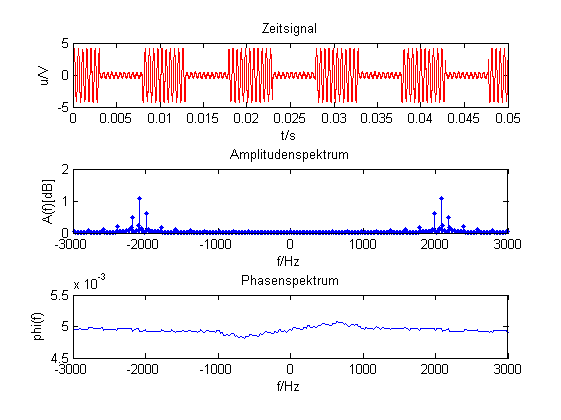
\includegraphics[scale=0.7]{Bilder/Am_Rec_2k_100Hz_mo}
                    \caption{gemessene Modulation eines Rechteck}
                \end{figure}
        
            \end{minipage}
        
        \end{tabular}
        \end{center}
        
        In Abb. \ref{fig:Sprache} ist die Modulation eines Sprachsignals zu
        sehen. Hierbei ist gut zu erkennen, dass die Nebenpeaks um die 2 kHz
        nicht den 100 Hz entsprechen, wie bei den ersten drei Signalen. Da ein
        Sprachsignal in einem breiteren Bereich von bis zu vier kHz liegt,
        streut das Sprektum hier mehr um die 2 kHz.
        
    \begin{figure}[H]
		\begin{center}
			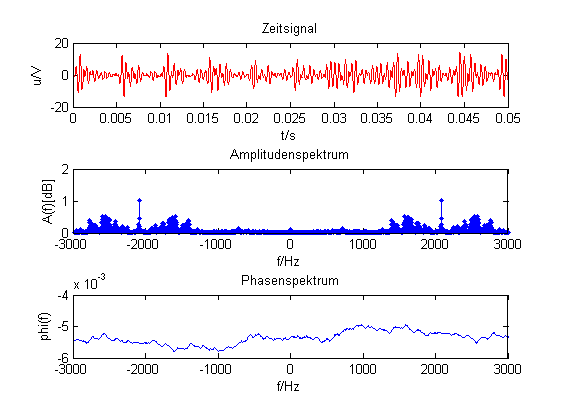
\includegraphics[width=0.8\textwidth]{Bilder/Sprachsignal}
		\end{center}
		\caption{Modulation eines Sprachsignals}
		\label{fig:Sprache}
	\end{figure}
        
        Bei der Demodulation werden zuerst die Signale ohne Tiefpass betrachtet.
        Dabei ergibt sich bei der Multiplikation mit dem selben Cosinus ein
        Cosinus Quadrat. Daher werden alle negativen Anteile nach oben geklappt
        und es gibt nur noch positive Anteile. Es sind auch noch mehrere
        Frequenzanteile enthalten, da der Cosinus mit der doppelt so hohen
        Frequenz (siehe Formel \ref{eq:demodulation}) nicht durch den Tiefpass
        gefiltert wurde.
      
         \begin{center}
        \begin{tabular}{ll}
        
        \hspace{-5cm}
            \begin{minipage}{0.67\textwidth}
                
                \begin{figure}[H]
                    \label{fig:DemocosinusoT}
                    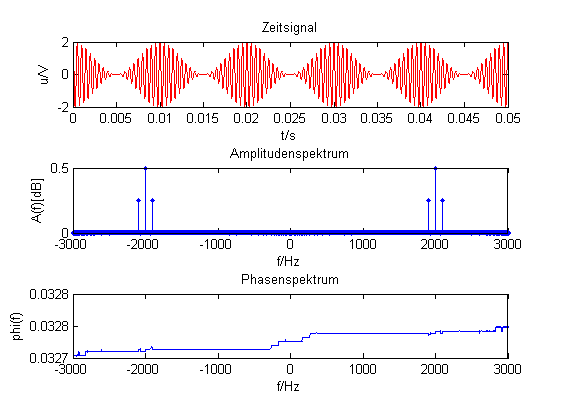
\includegraphics[scale=0.7]{Bilder/Am_Cos_2k_100Hz_mo}
                    \caption{gesendetes Signal}
                \end{figure}
        
            \end{minipage}
        
            \begin{minipage}{0.67\textwidth}
                \begin{figure}[H]
                    \label{fig:DemocosinusoT2}
                    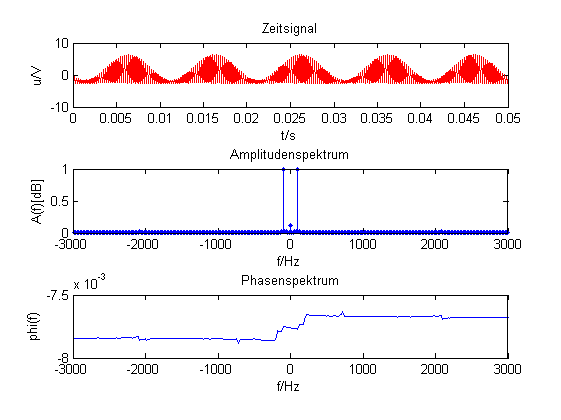
\includegraphics[scale=0.7]{Bilder/Demo_Sin_2k_100Hz_mo_ohneTiefpass}
                    \caption{empfangenes Signal}
                \end{figure}
        
            \end{minipage}
        
        \end{tabular}
        \end{center}
        
         \begin{center}
        \begin{tabular}{ll}
        
        \hspace{-5cm}
            \begin{minipage}{0.67\textwidth}
                
                \begin{figure}[H]
                    \label{fig:DemodreieckoT}
                    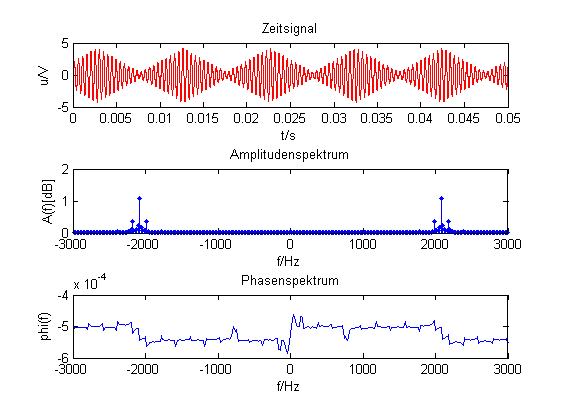
\includegraphics[scale=0.7]{Bilder/Am_Dre_2k_100Hz_mo}
                    \caption{gesendetes Signal}
                \end{figure}
        
            \end{minipage}
        
            \begin{minipage}{0.67\textwidth}
                \begin{figure}[H]
                    \label{fig:DemodreieckoT2}
                    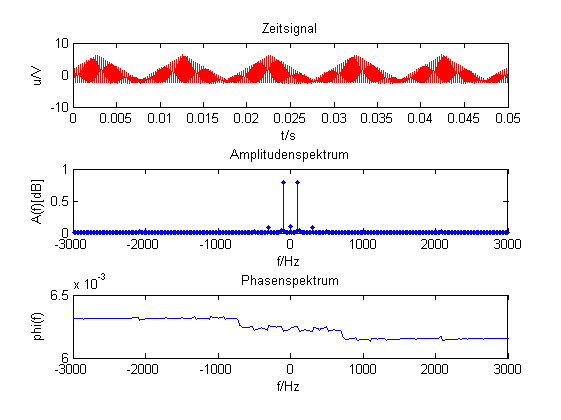
\includegraphics[scale=0.7]{Bilder/Demo_Dre_2k_100Hz_mo_ohneTiefpass}
                    \caption{empfangenes Signal}
                \end{figure}
        
            \end{minipage}
        
        \end{tabular}
        \end{center}
        
         \begin{center}
        \begin{tabular}{ll}
        
        \hspace{-5cm}
            \begin{minipage}{0.67\textwidth}
                
                \begin{figure}[H]
                    \label{fig:DemorechteckoT}
                    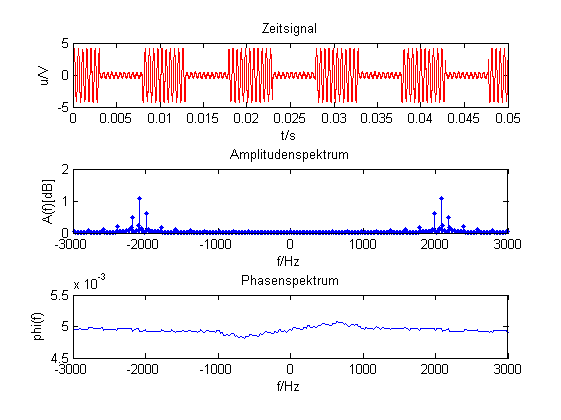
\includegraphics[scale=0.7]{Bilder/Am_Rec_2k_100Hz_mo}
                    \caption{gesendetes Signal}
                \end{figure}
        
            \end{minipage}
        
            \begin{minipage}{0.67\textwidth}
                \begin{figure}[H]
                    \label{fig:DemorechteckoT2}
                    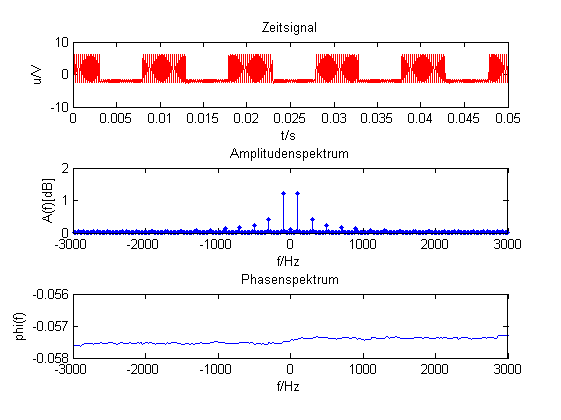
\includegraphics[scale=0.7]{Bilder/Demo_Rec_2k_100Hz_mo_ohneTiefpass}
                    \caption{empfangenes Signal}
                \end{figure}
        
            \end{minipage}
        
        \end{tabular}
        \end{center}
               
        Zuletzt wird der Tiefpass dazu geschaltet. Was passiert, wenn man die
        Grenzfrequenz variiert und sie noch zu hoch ist, kann man in Abb.
        \ref{fig:TPmitzugrosserGF} sehen. Das Signal ähnelt dem Basisbandsignal
        schon eher, als zuvor.
        
        \begin{figure}[H]
		\begin{center}
			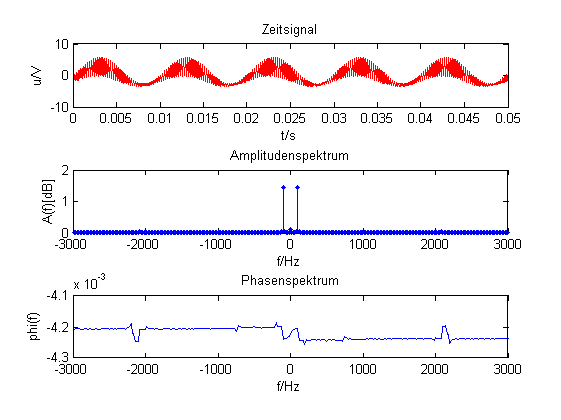
\includegraphics[width=0.8\textwidth]{Bilder/Demo_Sin_2k_100Hz_mo_mitTiefpasszugrosseGrenzfrequenz}
		\end{center}
		\caption{Demodulation mit Tiefpass mit zu großer Grenzfrequenz}
		\label{fig:TPmitzugrosserGF}
	    \end{figure}
	    
	    Mit einer niedrigeren Grenzfrequenz erhält man nahezu den Verlauf des
	    Basisbandsignals (Abb.). Die Abweichungen erklären sich dadurch, dass der
	    Tiefpass nicht eine unendliche Steilheit besitzt und nicht alle Frequenzen
	    über 100 Herz herausfiltert.
	    
	    \begin{center}
        \begin{tabular}{ll}
        
        \hspace{-5cm}
            \begin{minipage}{0.67\textwidth}
                
                \begin{figure}[H]
                    \label{fig:DemocosinusmT}
                    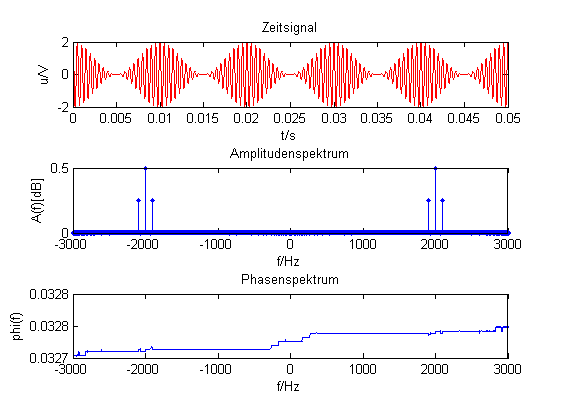
\includegraphics[scale=0.7]{Bilder/Am_Cos_2k_100Hz_mo}
                    \caption{gesendetes Signal}
                \end{figure}
        
            \end{minipage}
        
            \begin{minipage}{0.67\textwidth}
                \begin{figure}[H]
                    \label{fig:DemocosinusmT2}
                    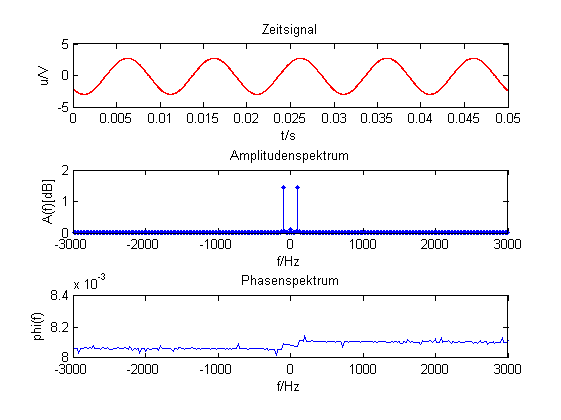
\includegraphics[scale=0.7]{Bilder/Demo_Sin_2k_100Hz_mo_mitTiefpass}
                    \caption{empfangenes Signal}
                \end{figure}
        
            \end{minipage}
        
        \end{tabular}
        \end{center}
        
        \begin{center}
        \begin{tabular}{ll}
        
        \hspace{-5cm}
            \begin{minipage}{0.67\textwidth}
                
                \begin{figure}[H]
                    \label{fig:DemodreieckmT}
                    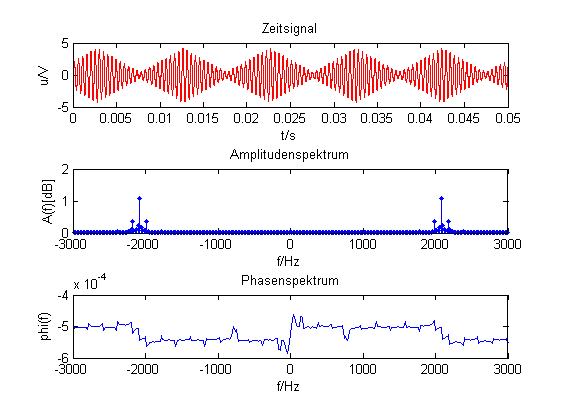
\includegraphics[scale=0.7]{Bilder/Am_Dre_2k_100Hz_mo}
                    \caption{gesendetes Signal}
                \end{figure}
        
            \end{minipage}
        
            \begin{minipage}{0.67\textwidth}
                \begin{figure}[H]
                    \label{fig:DemodreieckmT2}
                    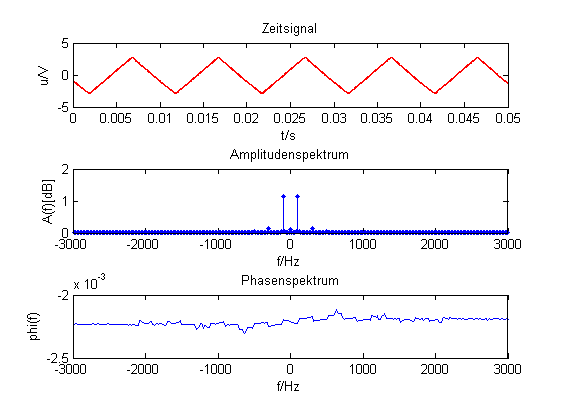
\includegraphics[scale=0.7]{Bilder/Demo_Dre_2k_100Hz_mo_mitTiefpass}
                    \caption{empfangenes Signal}
                \end{figure}
        
            \end{minipage}
        
        \end{tabular}
        \end{center}
        
        \begin{center}
        \begin{tabular}{ll}
        
        \hspace{-5cm}
            \begin{minipage}{0.67\textwidth}
                
                \begin{figure}[H]
                    \label{fig:DemodreieckmT}
                    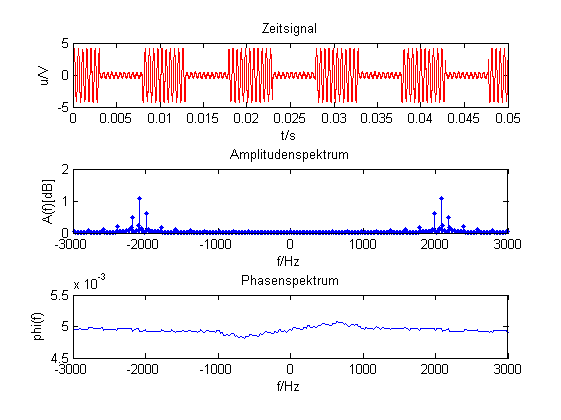
\includegraphics[scale=0.7]{Bilder/Am_Rec_2k_100Hz_mo}
                    \caption{gesendetes Signal}
                \end{figure}
        
            \end{minipage}
        
            \begin{minipage}{0.67\textwidth}
                \begin{figure}[H]
                    \label{fig:DemodreieckmT2}
                    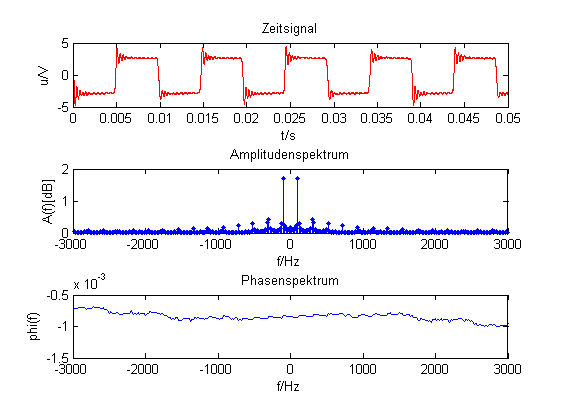
\includegraphics[scale=0.7]{Bilder/Demo_Rec_2k_100Hz_mo_mitTiefpass}
                    \caption{empfangenes Signal}
                \end{figure}
        
            \end{minipage}
        
        \end{tabular}
        \end{center}
        
    \end{quote}
    
\end{quote}


\section{FM}
\begin{quote}
    
    
    \subsection{Labordurchführung}
    \begin{quote}
        Wir haben im praktikum die FM-PFM-Umwandlung als Methode zur FM-Demodulation genutzt, da es ein relativ einfaches
        Verfahren ist. Hierbei wird das Signal zunächst durch einen Comparator in eine polare Rechteckfolge umgewandelt. Als
        Referenz für den Comparator wird \si{0}{\volt} eingestellt, damit jede positive Halbwelle des modulierten Signals zu
        einem positiven Rechteck wird und jede negative zu \si{0}{\volt}q.\\
        Anschließend wird das Signal noch durch einen Twin Pulse Generator geführt, der aus jeder steigenden Flanke ein
        Rechteckimpuls macht.\\
        Wofür der Twin Pulse Generator gebraucht wird ist leider weder aus dem Skrip ersichtlich, noch konnte es uns im Praktikum
        einleuchtend erklärt werden. Er wird wohl ``wegen irgendwelcher Feedback-Sachen oder so''\footnotemark gebraucht.\\
        Zuletzt wird das Signal noch tiefpass-gefiltert, um aus der Häufigkeit der Pulse wieder das Analoge ausgangssignal zu
        machen.
        \footnotetext{Aussage des Tutors im NUE-Praktikum am 16.05.2012}
        
        \TODO{egal: wir haben dann mehrere werte aufgenommen und \ldots auswirkungen \ldots tolle erkentnisse gewonnen}
    \end{quote}
    
    \subsection{Auswertung}
    \begin{quote}
        
        
        
        \subsubsection{Signalerzeugung}
        \begin{quote}
            \TODO{Thommy: wie haben wir die Frequenzmodulation auf dem brett gemacht?}
            
        \end{quote}
        
        
        
        \subsubsection{Trägerfrequenz $f_c$ \& Proportionalitätskonstante $K_{FM}$}
            
            
            
            \begin{center}
            \begin{tabular}{ll}
            
            \hspace{-4cm}
                \begin{minipage}{0.67\textwidth}
                    
                    \begin{figure}[H]
                        \label{fig:Tmax}
                        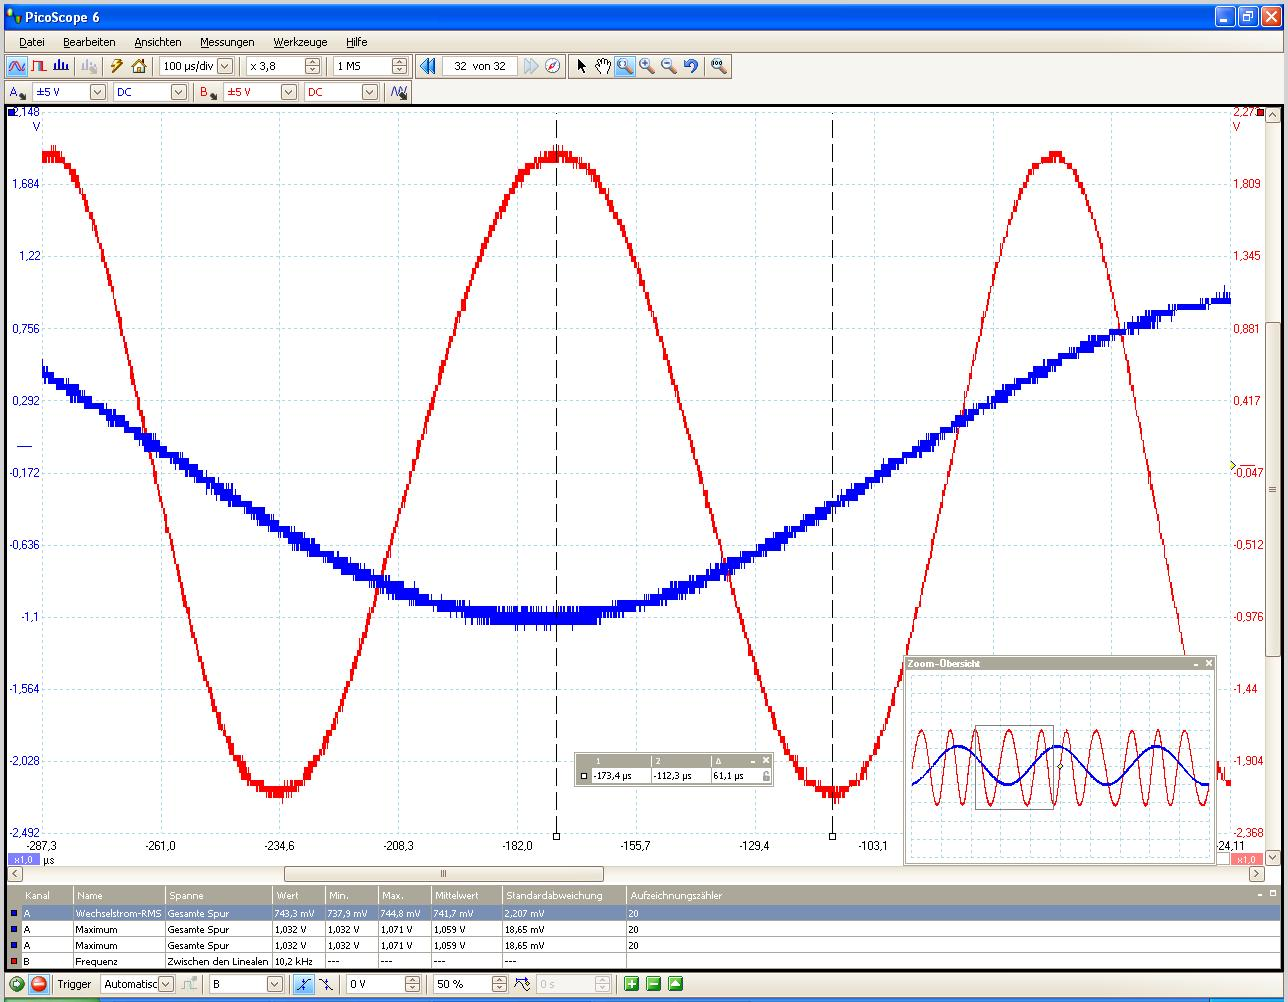
\includegraphics[scale=0.25, trim = 0mm 0mm 0mm 0mm, clip]{Bilder/Tmax}
                        \caption{Tmax = $61,1 \mu s$}
                    \end{figure}
                    
                \end{minipage}
                
                \begin{minipage}{0.67\textwidth}
                    \begin{figure}[H]
                        \label{fig:Tmin}
                        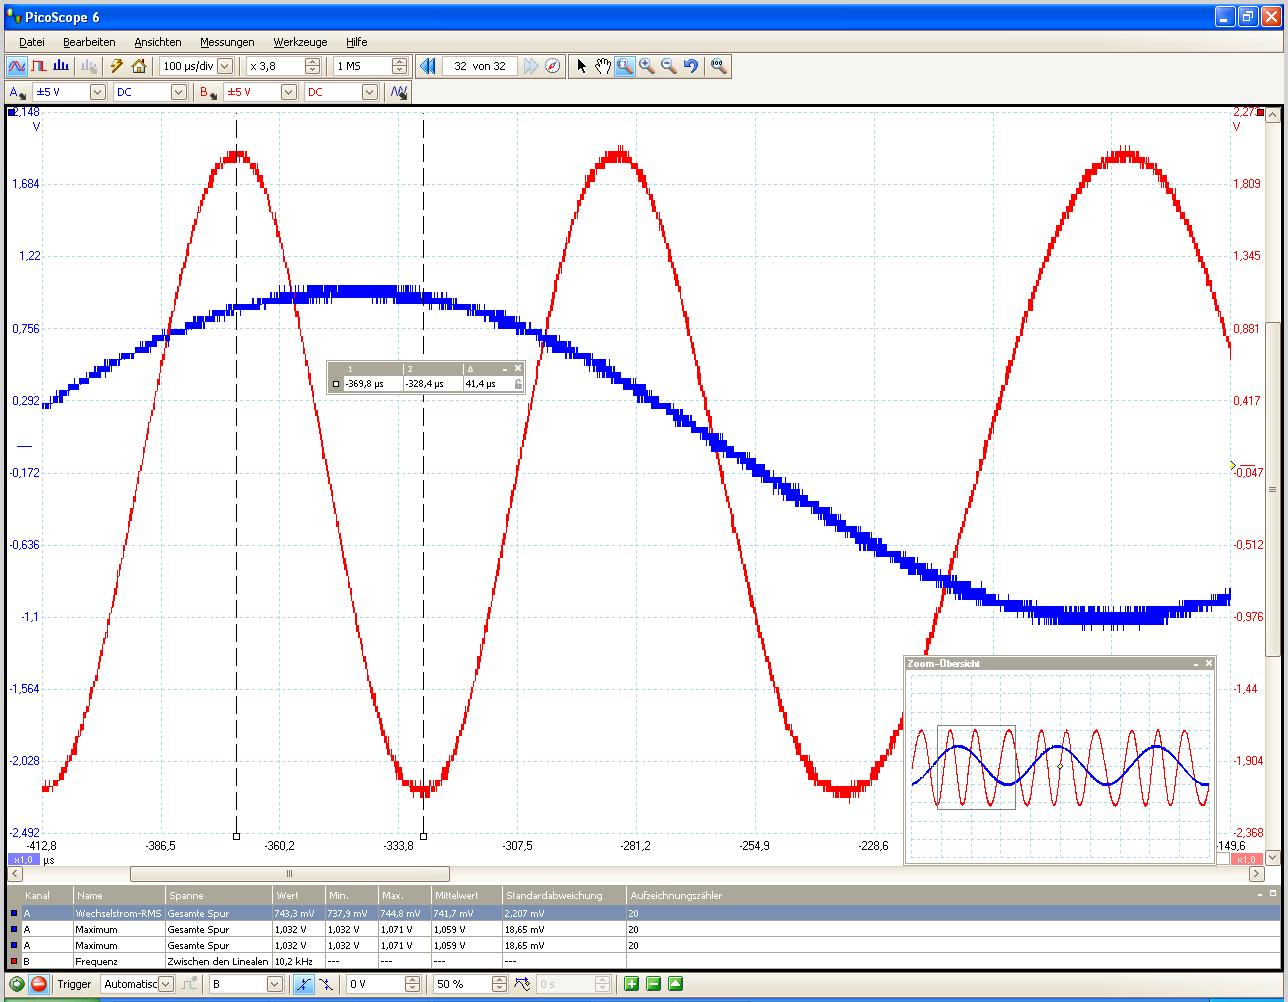
\includegraphics[scale=0.25, trim = 0mm 0mm 0mm 0mm, clip]{Bilder/Tmin}
                        \caption{Tmin = $41,4 \mu s$}
                    \end{figure}
                    
                \end{minipage}
            
            \end{tabular}
            \end{center}
            \vspace{2em}
            
        \begin{quote}
                
            Auf $K_{FM}$ kann man, bei bekannter Eingangsamplitude, mit der minimalen und maximalen Frequenz des modulierten
            Signals zurückschließen. Der Faktor $K_{FM}$ ist laut der FM-Modulationsformel \ref{equ:fm} proportional zur
            min-/maximalen Frequenz des Modulierten Signals bei min-/maximaler Amplitude des Nutzsignals.
            
            
            \begin{equation*}
            \begin{split}
            \\
                \Delta f_{max} &\approx \frac{1}{2} (\frac{1}{T_{min}} - \frac{1}{T_{max}})\\
                               &= \frac{1}{2} (\frac{1}{41,4 \mu s} -\frac{1}{61,1 \mu s})\\
                               &= 3894 \frac{1}{s}\\
            \\
                K_{FM} &=\frac{2 \pi \Delta f_{max}}{A_u}\\
                       &= \frac{2 \pi \p 3894 \frac{1}{s}}{1V}\\
                       &= 24467 \frac{1}{Vs}
            \\
            \end{split}
            \end{equation*}
            \label{equ:}
            
            Die Trägerfrequenz von \si{10}{kHz} lässt dich sehr gut an dem Folgenden Spektrum \ref{fig:freq_1k} (roter Plot)
            eines modulierten \si{1}{kHz} Sinus-Signals (blauer Plot) erkennen. Hier befindet sich die Mitte des Spektrums exakt bei
            \si{10}{kHz} woran sich die Trägerfrequenz ablesen lässt, da das Nutzsignal (der Sinus) das frequenzspektrum
            gleichmäßig nach rechts und links ausdehnt.
            
            \begin{figure}[H]
            \centering
                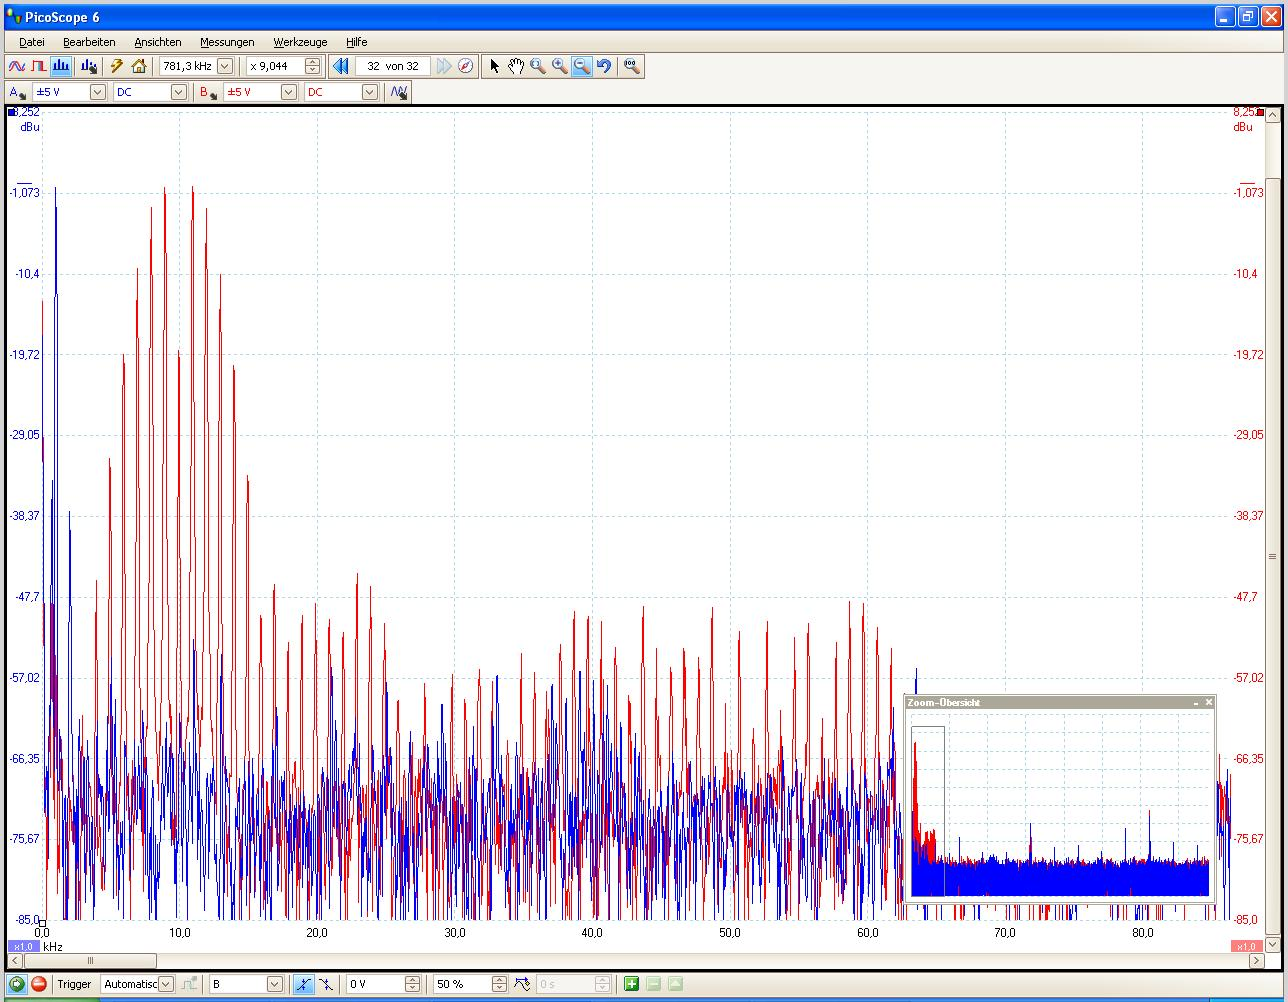
\includegraphics[scale=0.5, trim = 0.25cm 1.3cm 1cm 3.2cm, clip]{Bilder/freq_1k}
                    \caption{Frequenzmoduliertes 1kHz Signal}
                    \label{fig:freq_1k}
            \end{figure}
            
            
        \end{quote}
        
        \subsubsection{Auswirkung von Amplitude und Frequenz des Sendesignals auf das Ausgangssignal}
        \begin{quote}
            
            \begin{center}
            \begin{tabular}{ll}
            
            \hspace{-5cm}
                \begin{minipage}{0.6\textwidth}
                    \begin{figure}[H]
                        \label{fig:f50_05}
                        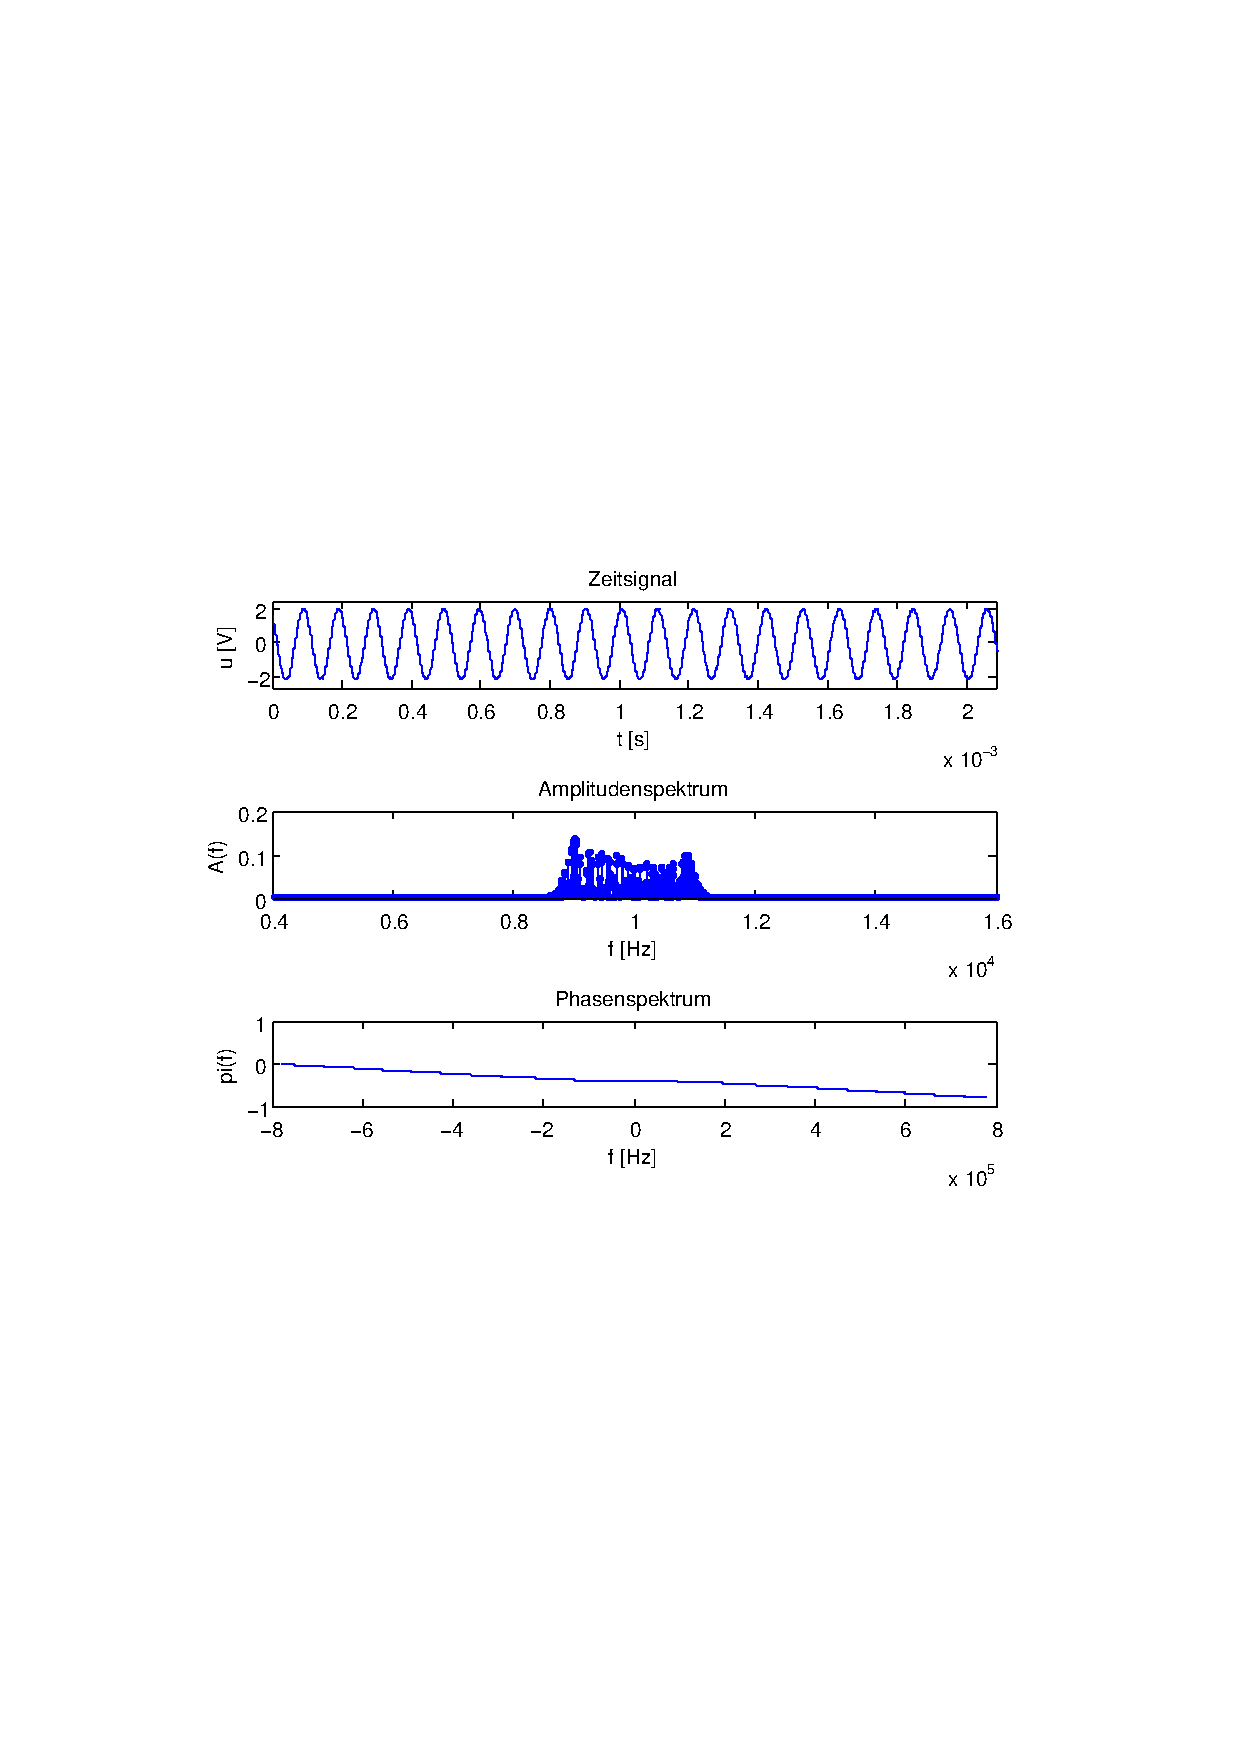
\includegraphics[scale=0.7, trim = 35mm 100mm 35mm 95mm, clip]{Bilder/f50_05}
                        \caption{f50_05}
                    \end{figure}
                \end{minipage}
                
                \begin{minipage}{0.6\textwidth}
                    \begin{figure}[H]
                        \label{fig:f50_1}
                        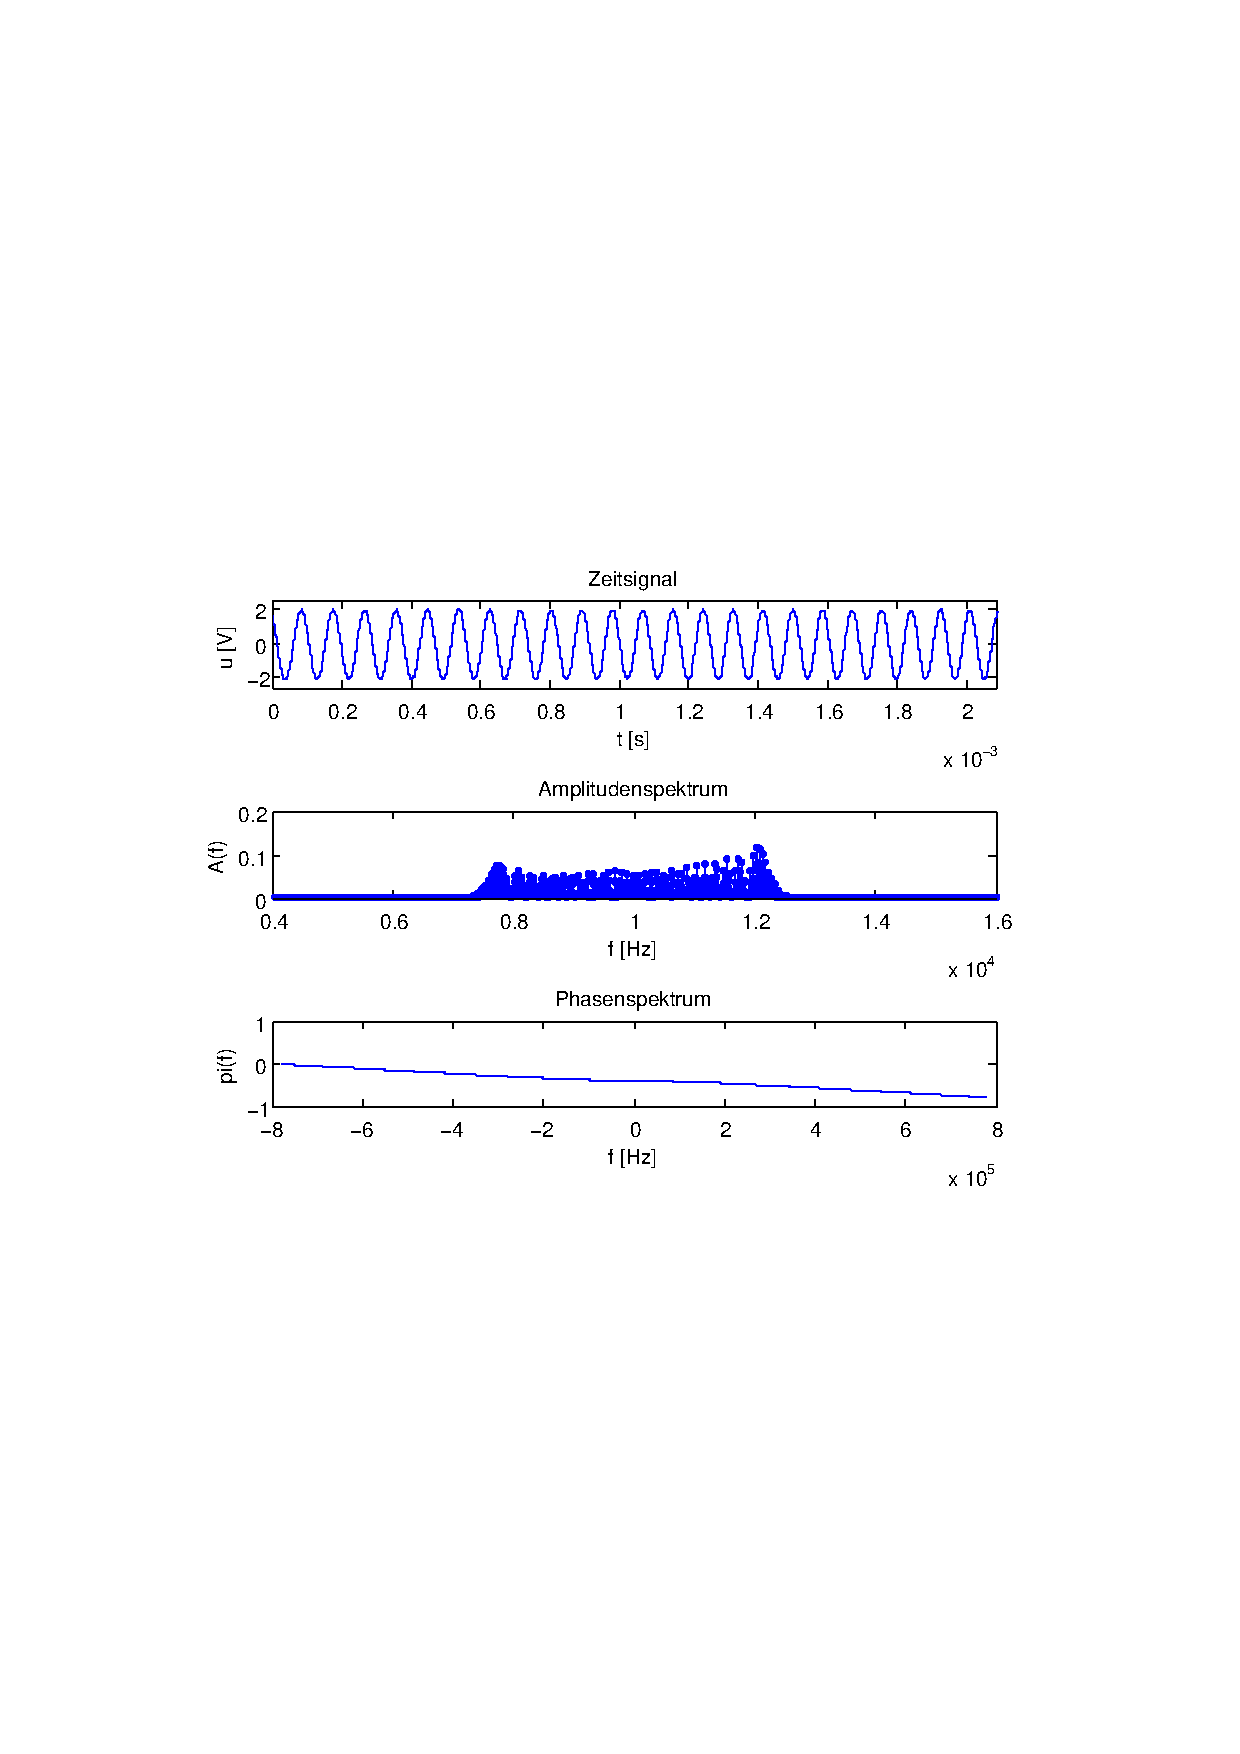
\includegraphics[scale=0.7, trim = 35mm 100mm 35mm 95mm, clip]{Bilder/f50_1}
                        \caption{f50_1}
                    \end{figure}
                \end{minipage}
            
            \end{tabular}
            \end{center}
            
            \begin{figure}[H]
            \centering
                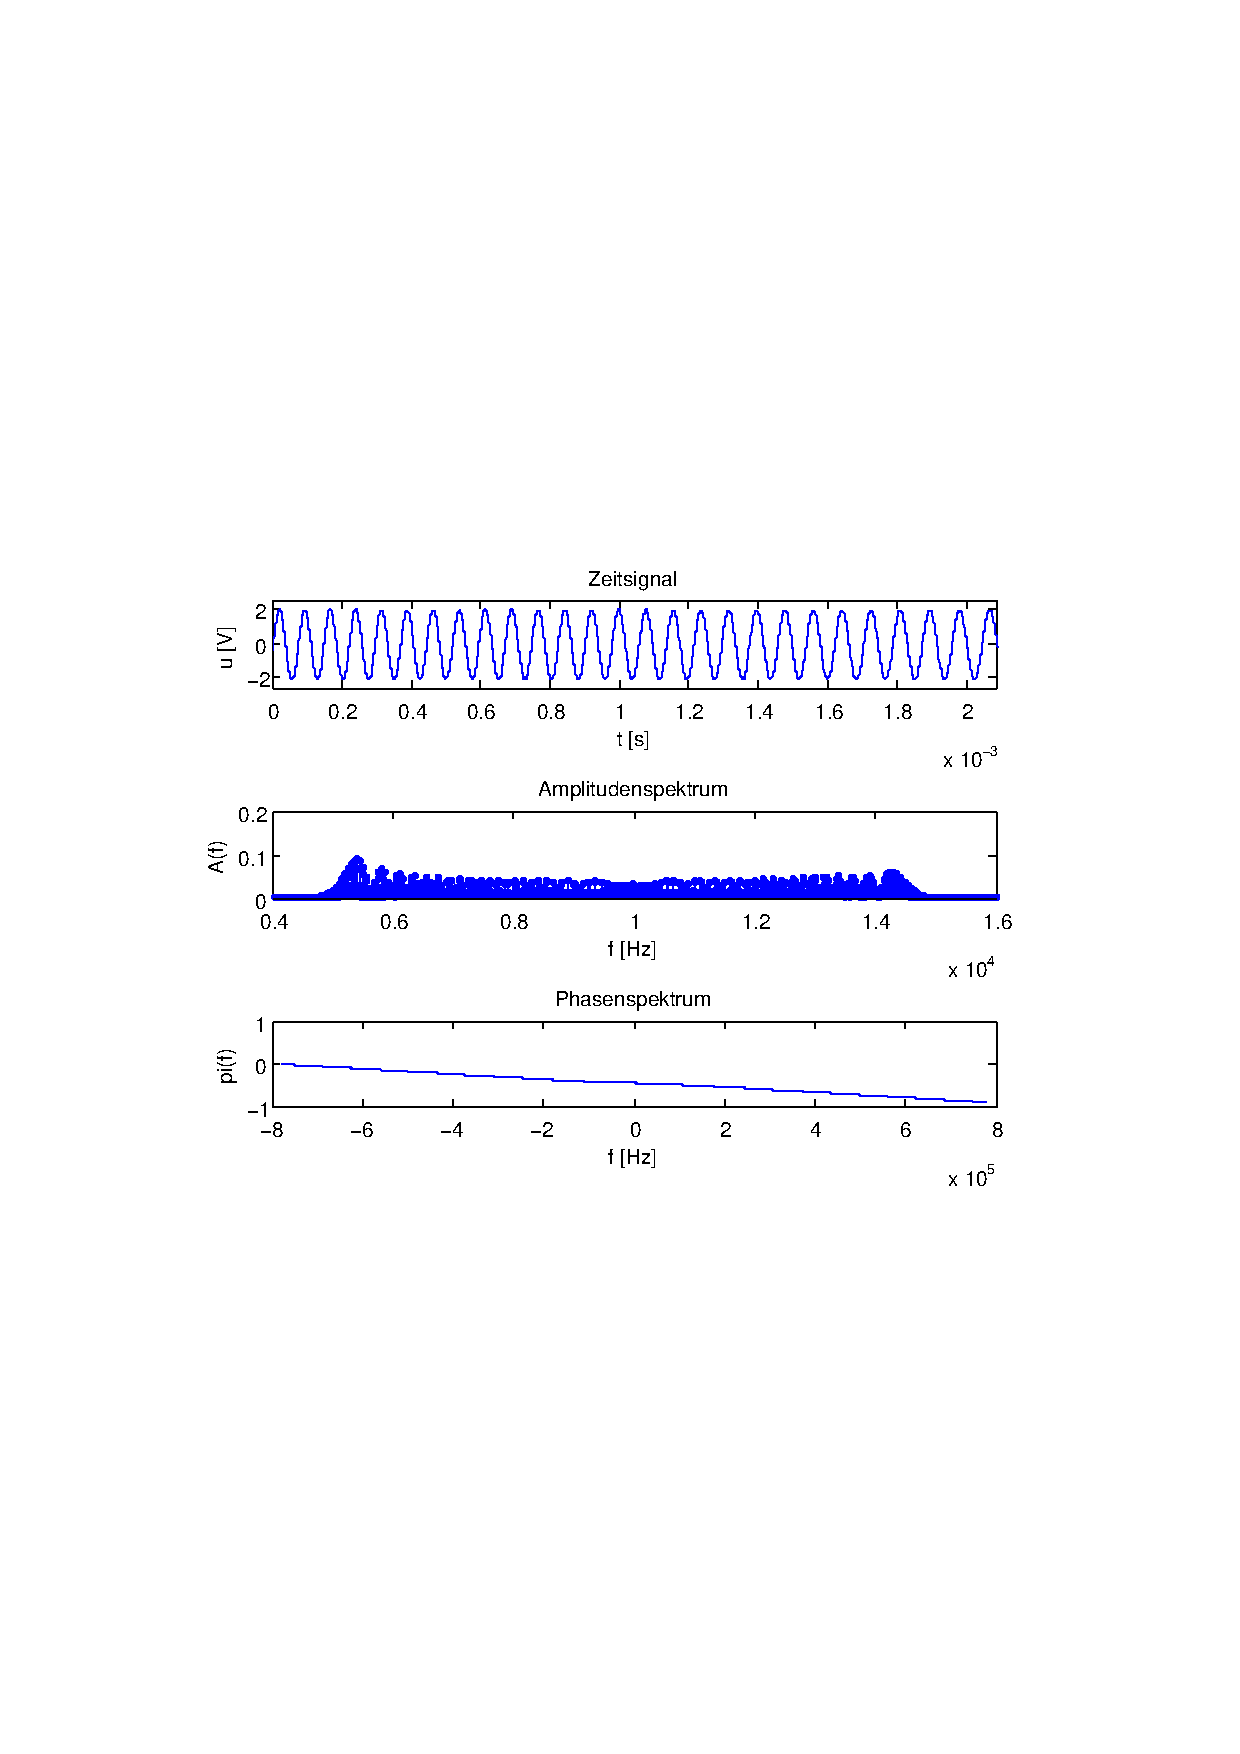
\includegraphics[scale=0.7, trim = 35mm 100mm 35mm 95mm, clip]{Bilder/f50_2}
                    \caption{f50 2}
                    \label{fig:f50_2}
            \end{figure}
            
            
            
        \end{quote}


        
        
    \end{quote}
    
    
    
    
    \subsection{Parkplatz}
    \begin{quote}
        
        Es ließ sich kein unterschied zwischen dem Signal nach dem Comparator und dem nach dem Twin Pulse Generator erkennen. Das
        liegt wahrscheinlich daran, dass die Trägerfrequenz sehr hoch ist und der Puls des Twinpulse-Generators mit
        \SI{5}{\micro\second} ähnlich breit ist wie eine Halbwelle des modulierten Signals.
        
        frequenzhub
        trägerfrequenz
        signalfrequenz
        $\beta$
        Basisband
        
    \end{quote}
    
\end{quote}



% \begin{quote}
%     \lstinputlisting[
%         caption={Scilab-script},
%         label=lst:scilab]
%         {./Scilab/Motor.sce}
%         
% \end{quote}

%--------------------------------------------------------------------
%--------------------------------------------------------------------
% \begin{thebibliography}{999}
% 
% \bibitem{Boris}Boris Henckell: Ein Paar sachen geklaut.. ähhh inspirationen geholt
% \href{http://www.krachler.com/fileadmin/user_upload/arbeiten/Reglersynthese_Christian_Krachler.pdf}{Reglersynthese nach dem Frequenzkennlinienverfahren}, S16, S22, 08.05.2012
% 
% 
% %Name, Vorname.; evtl. Name2, Vorname2.: Titel des Dokumentes
% %oder Buches, Zeitschrift/Verlag/URL (Auflage, Erscheinungsort, -jahr), ggf. Seitenzahlen
% %\bibitem [Wiki10] {DigitaleMesskette2} \url{www.wikipedia.org}, Zugriff 22.03.2010
% \end{thebibliography}


\end{document}
